\documentclass{article}
\usepackage{textcomp}
\usepackage[utf8x]{inputenc}
\usepackage{graphicx}
\graphicspath{ {problem4/} }

\title{Laboratory No.1 at MS}
\author{gr. FAF-161 st. Polina Gore}

\begin{document}

  \begin{titlepage}

    \newcommand{\HRule}{\rule{\linewidth}{0.5mm}} % Defines a new command for the horizontal lines, change thickness here

    \center % Center everything on the page

    \textsc{\LARGE UTM}\\[1.5cm] % Name of your university/college
    \textsc{\Large MS}\\[0.5cm] % Major heading such as course name

    \HRule \\[0.4cm]
    { \huge \bfseries Laboratory No.1}\\[0.4cm] % Title of your document
    \HRule \\[1.5cm]

    \begin{minipage}{0.4\textwidth}
      \begin{flushleft} \large
        \emph{Student:}\\
        Polina \textsc{Gore} % Your name
      \end{flushleft}
    \end{minipage}
    ~
    \begin{minipage}{0.4\textwidth}
      \begin{flushright} \large
        \emph{Supervisor:} \\
        Victor \textsc{Turcanu} % Supervisor's Name
      \end{flushright}
    \end{minipage}\\[4cm]

    \vfill
    
    {\large \today}\\[3cm]

  \end{titlepage}

  \pagenumbering{gobble}

  \newpage
  \pagenumbering{arabic}

  \section{Problem 1}

    \subsection{At the hospital}

    The psychologist Tversky and his colleagues say that about four out of five
    people will answer (a) to the following question:

    A certain town is served by two hospitals. In the larger hospital about 45
    babies are born each day, and in the smaller hospital 15 babies are born each
    day. Although the overall proportion of boys is about 50 percent, the actual
    proportion at either hospital may be more or less than 50 percent on any day.
    At the end of a year, which hospital will have the greater number of days on
    which more than 60 percent of the babies born were boys?

    (a) the large hospital;

    (b) the small hospital;

    (c) neither, the number of days will be about the same.

    Assume that the probability that a baby is a boy is .5 (actual estimates
    make this more like .513). Decide, by simulation, what the right answer is to
    the question. Can you suggest why so many people go wrong?
    \subsection{Solution}
    The function `oneDayHosp(kids)' takes as a
    parameter the number of babies born in a hospital and returns 1 if the
    probability is higher than 60\% in one day.

    In a for loop we iterate over 365 days, and add the returned value of the
    function oneDayHosp to the 2 variables
    `largeHdays' and `smallHdays', which obviously are the number of days with
    a probability higher than 60\% in the large hospital and respectively in
    the small hospital.

    Then we compare the results, which gives us the answer (b) most of the time.

  \newpage

  \section{Problem 2}

    \subsection{I bet my life on this one}

    \hspace{6mm}Are you still in mood for gambling? Why don\textquotesingle t
    we get more serious then!\\Let\textquotesingle s roll old school and play
    some Russian roulette. Here\textquotesingle s the deal. I have a revolver
    with a 6 slots barrel and only 2 bullets. Now I put the bullets into the
    revolver in adjacent slots, spin the barrel and hand you the gun. You point
    the gun to your head. You pull the trigger and . . . Click!
    you\textquotesingle re still alive. Congratulations but the game is not
    over yet. You have to pull the trigger one last time.
    Now you have two choices.

    1. You spin the barrel afterwards you pull the trigger.

    2. You pull the trigger without spinning.

    Luckily you also have a computer in front of you so you\textquotesingle re
    allowed to simulate the current situation such that you can make a better
    decision.

    Your task is to find the probability for both cases. After
    you\textquotesingle ve computed the probability for the initial conditions
    please also find out what are the probabilities in case the bullets
    are not adjacent.

    After you\textquotesingle re done with that, compute the same probabilities
    only when the gun has a 5 slots barrel and 2 bullets. At the end you have
    to present the result for 8 different outcomes. Good luck staying alive.

    \subsection{Solution}

    \hspace{5mm} First of all, imagine the barrel as a circular array ex:
    [1,0,0,0,0,1]

    1 - bullets, 0 - empty slots, here - adjacent bullets.

    The function `findProcent' computes for 1000 cases the probability of being
    dead after the second shot, then returns the probability of being alive\\
    (P(~A) = 1 - P(A))

    This function is called 8 times with different arguments, for 6 or 5 slots
    in the barrel, where we can have adjacent or non-adjacent bullets and with
    option to spin or not.

  \newpage

  \section{Problem 3}

    \subsection{Catch them all}

    \hspace{5mm}Assume that every time you buy a box of Chio (a moldovan brand
    of chips), you receive one of the pictures of the n of the members of
    the NOROC band. Over a period of time, you buy m ≥ n boxes of Chio.
    Write a computer program to compute the probability that you get all
    n members of NOROC. Use this program to find, for given n, the smallest
    value of m which will give probability ≥ .5 of getting all n pictures.
    Consider n = 50, 100, and 150 and show that\\ m = n log n + n log 2
    is a good estimate for the number of boxes needed.

    \subsection{Solution}

    For any input n - number of members in Noroc band, we find the minimum `m',
    m ≥ n, m - number of chips Chio whith 1 photo of 1 member from n members.
    For this, we compute for 1000 cases, with the help of the function getResult,
    which returns the number of boxes needed to find all photos (which is always
    for probability == 1, not bigger than  0.5, - disadvantage).

    Then, we see that the number we found is almost the same as the estimated one.

  \newpage

  \section{Problem 4}

    \subsection{Dangerous pixels}

    \hspace{5mm}This morning CIA faxed UTM the following map scan. The total captured
    surface is around 42 square miles (duh . . . this imperial metric).\\ With red is
    marked the land that is mined by the guerrilla forces.\\ Now CIA needs to evaluate
    the logistics required to defuse the deadly mines.\\ But of course they do not have
    enough resources to compute the red area.\\ Which is why they are playing their
    trump card - the brilliant engineers from FAF-161.

    The stakes are very high, and lots of innocent lives can be spared. So please
    compute the mined area a.s.a.p., using Monte Carlo method.

    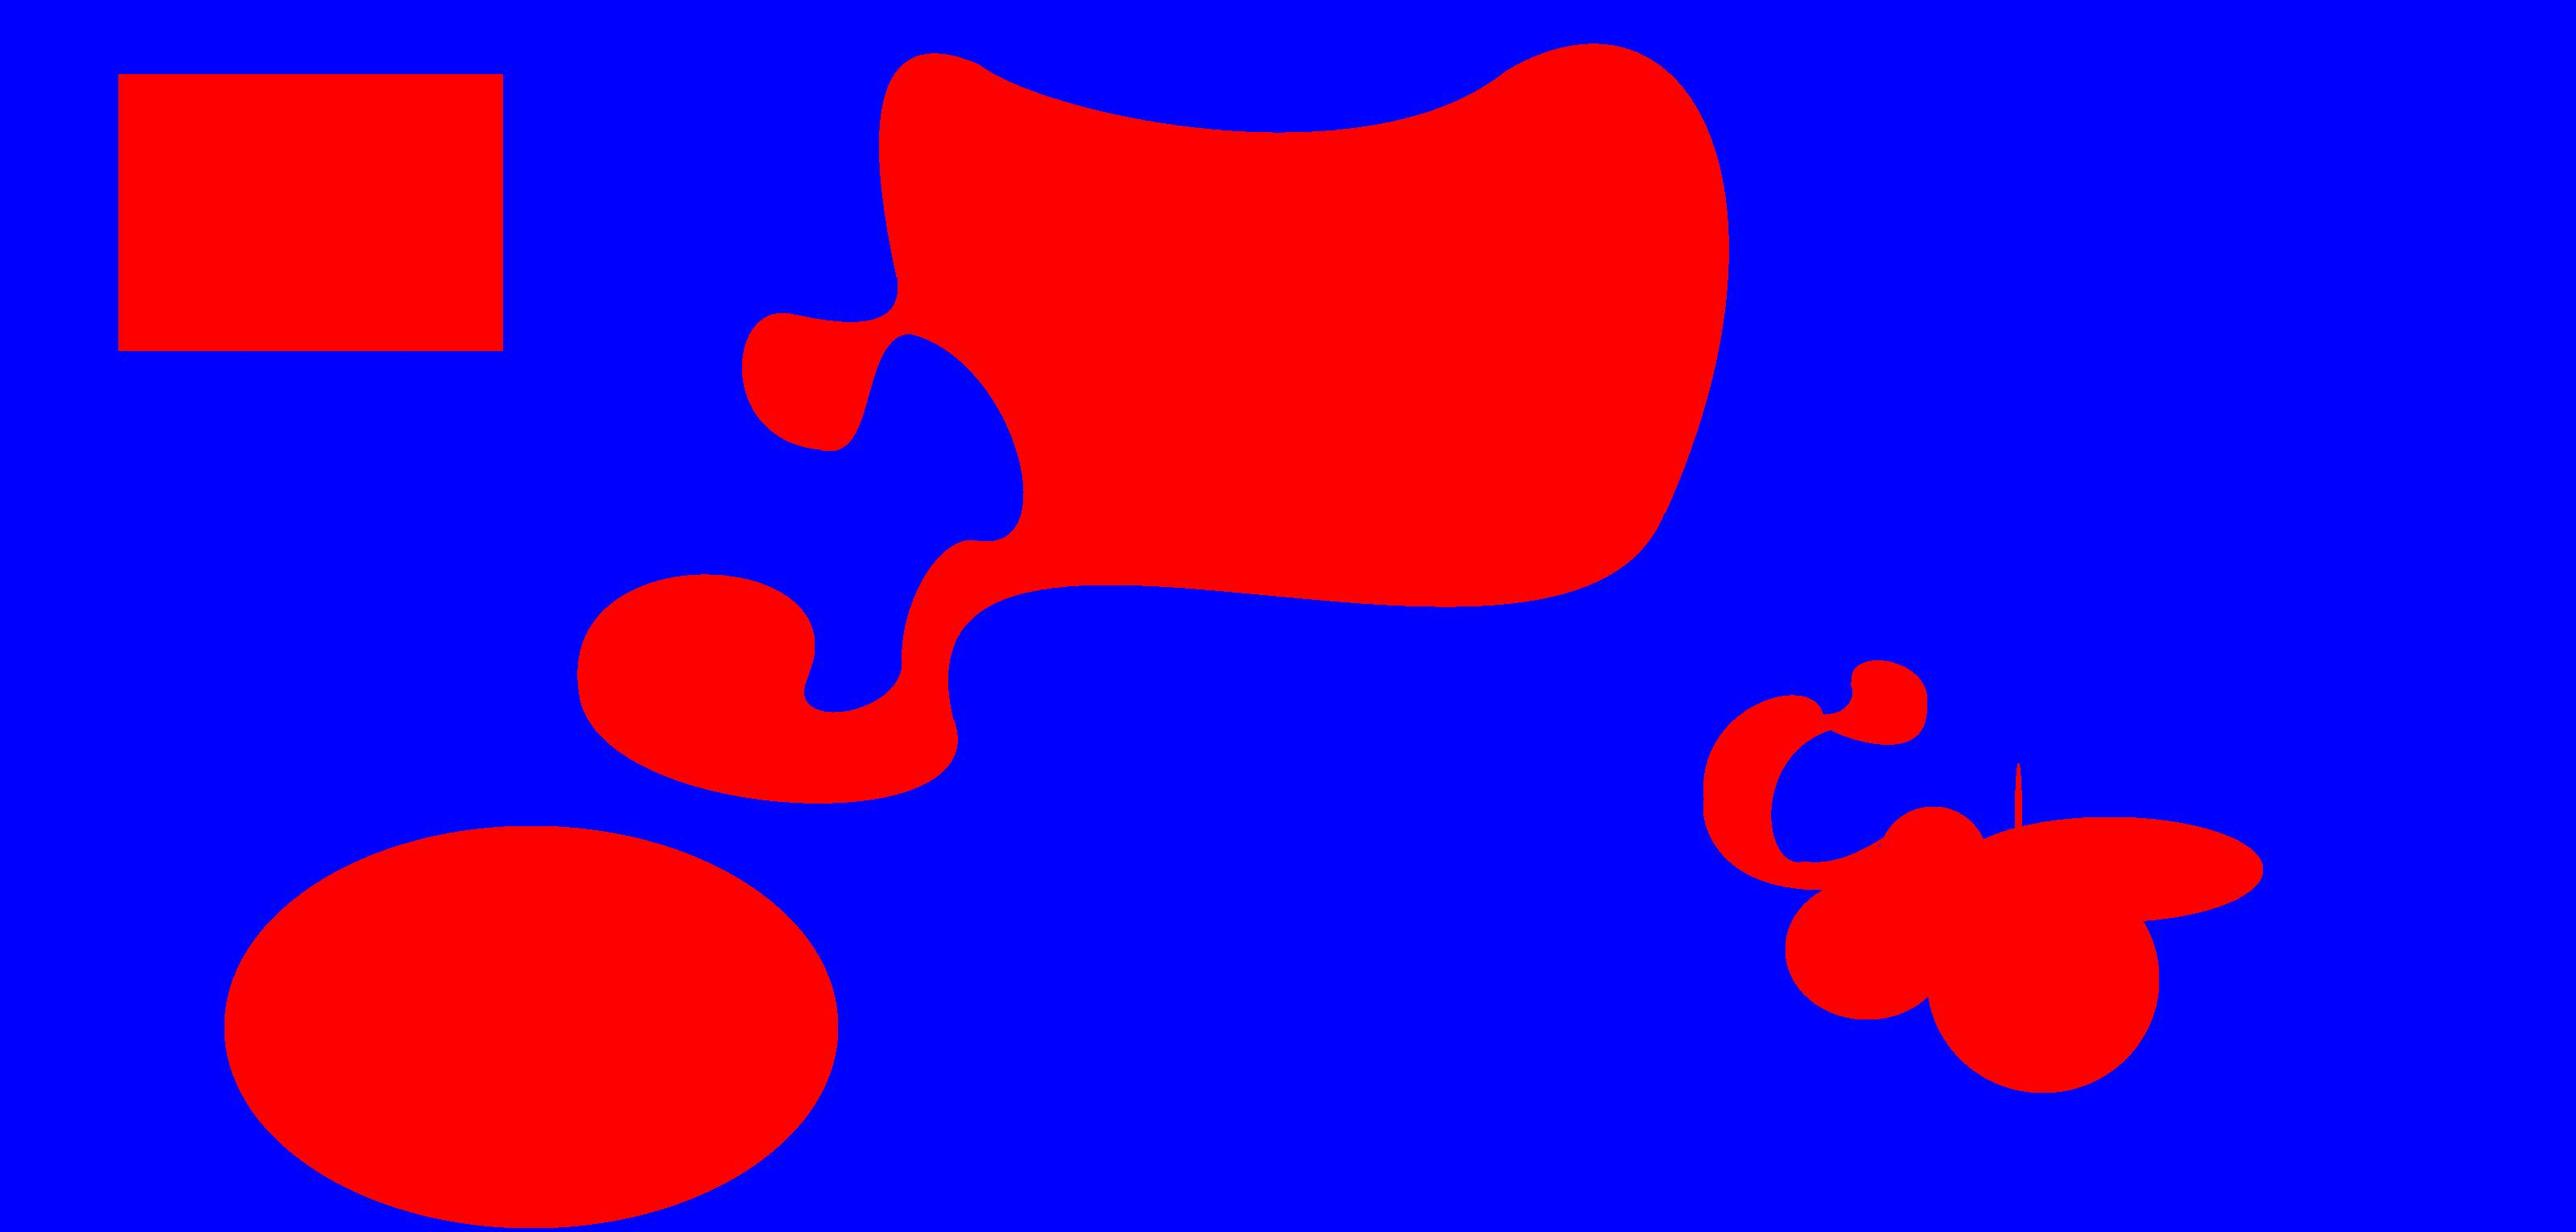
\includegraphics[scale=0.1]{forlab}

    \subsection{Solution}

    \hspace{5mm}For this problem, I used the pillows library as sugested.

    To compute the mined area, we take a a random tuple (x, y) which is a
    coordinate, and check if the pixel at that coordinate is red, adding 1 to
    areaRed if True.

    It is done for 100k cases, and the returned value is the area of the
    dangerous zone.

    The red area is 10-11 miles.

  \newpage

  \section{Problem 5}

    \subsection{Let’s get serious and crack something}

    \hspace{5mm}This exercise aims to introduce you to very basic concept of
    hashing algorithms, how they work, why are they useful and what are their
    weaknesses.\\ And along the way you’ll pick up the principle behind the
    flaw of hashing functions.

    Now you’re face to face with md5 hashing algorithm. Your task ahead is
    to find collisions for this algorithm, (only for the first 40 bits of the hash, aka
    first 10 hex characters). For that purpose you’re going to use birthday attack,
    that is based on birthday paradox.

    You have to write a small program that would eventually find a collision for
    the first 40 bits generated generated by md5 algorithm.

    \subsection{Solution}

    \hspace{5mm}The concept behind this problem is really simple, but to
    obtain a valid result is a pain in the ass.

    In this program we have to find a collision for the first 40 bits of the
    hashes of 2 different inputs.

    I chose the uuid4 function, because it gives unique random strings.\\
    So, when the first 10 hex characters collide (are equal) then it is a
    collision.

    The problem is that it takes a long period of time.\\
    For the first 8 hex chars it takes 10-30 min, while for the first 10,
    it takes longer than 3-4 hours.

\end{document}
